\section{Comparison Matrices}\label{sec:matrix}

In this paper, we propose three matrices to assist the architect in his task of selecting the right technologies for his use-case. To achieve this, we classify technologies that help to build Semantic REST systems along criteria that are categorized by the levels of WS3. As we showed in the previous section, the WS3 classification is too coarse-grained to grasp all important differences between systems of the same maturity level. Therefore, presented matrices compare the technologies along a set of precise criteria to highlight these differences. Some criteria cannot be linked to one level of WS3 but remain useful so we decided to place them in a "other" category.

In this section we present the methodology that we followed to select the technologies and classification criteria, we present the matrices and leverage them to draw a high-level comparison of the technologies.

Among available technologies, we distinguished three categories: (i) Interface Description Languages (IDL), (ii) data-interchange formats and (iii) implementation frameworks. One matrix is presented per category.

\subsection{Comparison Matrices Design Methodology}

% TODO - IN PROGRESS - From reviewer 2 : My impression is that the paper only accounts the result of the web search, and developers' expertise is not actually leveraged. Which are the daily problems developers face? Go deeper with their experience. The framework is intended to be used by developers, you should take into account their insights from the trenches. Interview people from your company if needed, and provide links to their responses/questionnaires.

% TODO - From reviewer 2 : The methodology steps can be shortened, as they do not add any useful information. How did you verified the criteria (step v) w.r.t. your previous projects? Provide an example.

% TODO - From reviewer 1 : Section 4.1: The section present a way to select papers, but it is not clear how to select papers concretely. The last three paragraphs in Section 4.1 should be expanded.

The design of the comparison matrices follows a 5 steps sequential process: (i) looking for candidate technologies, (ii) selecting candidate technologies, (iii) deep reading of each candidate technology, (iv) elaboration of fine grain criteria to characterize and differentiate technologies, (v) double-verification that the elaborated criteria highlighted the differences between technologies.

The research of candidate technologies (step i) was done by:

\begin{enumerate}
    \item Searching Google and Google Scholar for Semantic REST Technologies using compositions of keywords from the set: ["web", "semantic", "restful", "rest", "service", "API", "interface", "description", "documentation", "language", "modeling", "hypermedia", "document", "format", "RDF", "data-interchange", "linked data", "hateoas", "rest api", "framework"];
    \item Searching Google Scholar for tools automating tasks from services description, using keywords: "matchmakers", "service composition", "service discovery", "rest service analysis", "automated mashups", we then selected other papers and technologies from their references and the papers that cite those we selected;
    \item Looking at the proceedings of ICWE and WS-REST. 
\end{enumerate}

% Maybe update the 81 number below if the Github with raw material changes.
From these researches, we selected 81 papers, standards, articles and web pages (step ii) from their abstract or introduction. We selected documents that were the specification of an interface definition language or model, a framework that supports HATEOAS features, an interchange format that supports RDF or HATEOAS features, a comparison between these technologies or a tool leveraging them. Frameworks to build Semantic Web Services were excluded because they are based on triples which are too far from the resource-oriented design of REST. We opened our research to technologies from the 1990s to today and retained technologies that are still available today.

As a next step, we read the specification of each chosen technology (step iii) and elaborate classification criteria (step iv). Some criteria targeting interchange formats are the H Factor\footnote{\url{http://amundsen.com/hypermedia/hfactor/}}. Others were carefully designed to highlight differences between technologies in the area of Semantic REST, based on the core design of the technologies, the features they provide and the details of the WS3 maturity model. Several steps of refinement were needed to avoid duplicating criteria or hiding important details. All the raw material used to elaborate this classification is available online\footnote{\url{https://github.com/AntoineCheron/semantic-restful-api-technologies-comparison-matrix}}. 
% TODO @Johann @Olivier: the above paragraph needs to be reviewed. If not good enough, I will need help to improve it.

As a final step (step v), we read the specifications again to verify results and validate  that the selected criteria highlighted differences and commonalities well.

\paragraph{Popularity criteria}

% Long version
%We included a popularity criteria to offer a vague idea of whether a community might help with any problem that may arise and how likely the technology will be lasting. The popularity score is between 0 and 2. The highest, the more popular the technology is. To score technologies we took several indicators into account. First, the number of questions about the technology on Stack Overflow\footnote{\url{https://stackoverflow.com}}. Then, for IDL and interchange formats only, we looked at the five most popular libraries on NPM\footnote{\url{https://www.npmjs.com/}} and Maven Central\footnote{\url{https://mvnrepository.com/repos/central}}. On NPM we selected the weekly downloads and on Maven, the usages. On the other hand, for the frameworks we collected the total downloads from the main repository of its language. The popularity score is computed as follows:

%Short version
We included a popularity criteria to offer a vague idea of whether a community might help with any problem that may arise and how likely the technology will be lasting. The popularity score is between 0 and 2. The highest, the more popular the technology is. It is computed as follows:

\begin{itemize}
    \item 0 - Not enough to reach 1
    \item 1 - More than 100 questions on stack overflow AND (2500+ NPM weekly downloads OR 100+ maven usages)
    \item 2 - More than 400 questions on stack overflow AND (more than 500.000 total downloads OR more than 15.000 NPM weekly downloads OR more than 500 maven usages)
\end{itemize}

\subsection{Interface Description Languages}

Interface Description Languages (IDLs) provide a vocabulary to document domain, functional and non-functional aspects of an API. We identified 16 candidates that are classified according to 31 criteria in Fig~\ref{idl-matrix}.

When IDLs and data-interchange formats are both compatible with RDF, they can be combined to form a file format usable as both the data-interchange format and the IDL. This has great benefits to lower the overall complexity and increase the evolvability of the system.

\subsubsection{Selected technologies}

Among the classified IDLs, 4 are meta-models from conference papers.
In \cite{Rapido} authors present a tool to sketch CRUD or Hypermedia APIs. On the Hypermedia APIs mode, the user sketches the application using state machines and then obtain a description in the HAL or Collection+JSON format.
\cite{Schreier:2011:MRA:1967428.1967434} models each resource type as a finite state machine with deterministic state transitions. In this model, each resource type has a single initial state, operations can go beyond CRUD and conditions can be used to inform the availability of operations. However, conditions are not modeled in more details, which does not make them machine-interpretable.
In \cite{10.1007/978-3-642-22233-7_24}, authors propose to model the system as a non-deterministic state machine. This method makes software agents unable to discover the set of messages to exchange in order to make an operation available. Haupt et al.
\cite{10.1109/ICWS.2014.30} propose a thorough multi-layered model that separates the domain model from the URI model. It does not allow specifying conditions on the availability of operations and see resources as having a static structure, making it impossible to represent different state of a resource with different classes. 

The 11 other interface description languages we found are open-sourced projects or W3C recommendations. They are listed in Fig~\ref{idl-matrix}.

% FIGURE OF THE IDL CLASSIFICATION
\begin{figure*}[!ht]
\caption{Interface Description Languages Comparison Matrix}
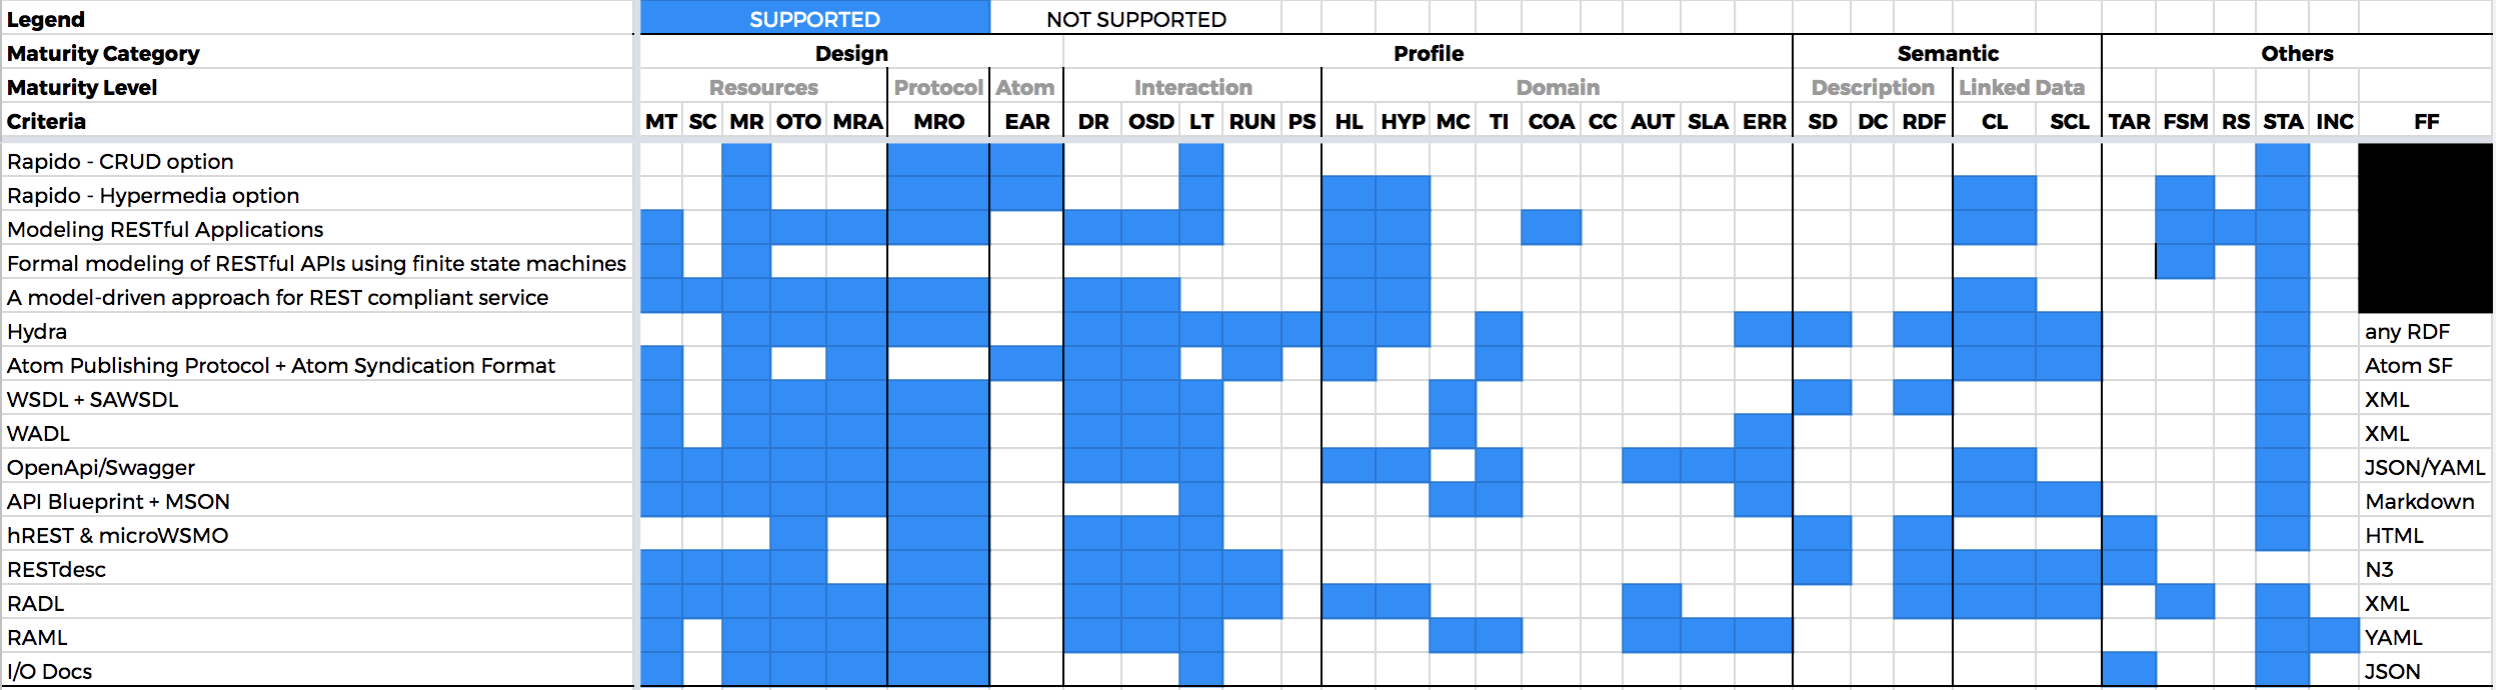
\includegraphics[width=1\textwidth]{figures/IDL.png}
\label{idl-matrix}
\end{figure*}

\subsubsection*{Synthesis}

% @Johann and @Olivier : I'd like to have your point of view on what is interesting and what is not among these conclusions

First, the matrix highlights the fact that most technologies help building mature systems on the \textit{design} dimension and \textit{interaction profile} level of the \textit{profile} dimension, D3-P1 in the terms of WS3.
On the other side when we look at the \textit{semantic} dimension, we notice that five out of sixteen technologies support the use of RDF vocabulary, which allows to build Linked Data compatible APIs. As a reminder, this is required to build Semantic REST systems.
Moreover, by supporting the use of RDF vocabulary, IDLs can be enriched with other vocabularies in order to reach a higher level of maturity.

Among the technologies, four can be distinguished by the number of criteria they meet: Hydra (18), RADL (18), OpenAPI (17) and RESTdesc (17).
OpenAPI is the only one that has no support for RDF. Thus, it helps in building systems up to D3-P2-S0 on the WS3 scale.
On the other hand, Hydra, RADL and RESTdesc support the use of RDF vocabulary, which makes these technologies better suited to build systems that are mature on the semantic dimension.

\paragraph{Towards HATEOAS APIs}
From the matrix we notice that most technologies target the documentation of the API in a single, non-splittable file. Hence, they are not suited to provide hypermedia controls at runtime.

% Antoine - C'est un point que je trouve personnellement intéressant mais je ne suis pas sur qu'il ait sa place dans le papier
On the other hand, only one approach, \cite{Schreier:2011:MRA:1967428.1967434}, supports the description of the conditions that determine the availability of a link, and no one makes this meta-data machine-interpretable. This makes software agents unable to find a way to make an operation available when it is not.

\paragraph{Towards better-documented APIs}
Only four technologies support the addition of business constraints to the models although it lowers coupling and improves user experience. For example with the automatic generation of forms with client-side validation.

Finally, we note that most scientific publications recommend the modeling of RESTful systems as state machines whereas most open-sourced or W3C IDL authors don't consider this design method. And yet, the use of deterministic state machines eases determining the availability of operations on a resource.

\subsection{Data-interchange formats}

Data-interchange formats provide a data-structure, a vocabulary and a layout to represent a resource and its meta-data at runtime. When the goal is not to provide meta-data, JSON, XML and YAML are the three formats the most widely used in the industry.

On the other side, when the system to build have to send meta-data, no interchange format is considered as a standard today. We selected 11 candidate technologies, which are classified in Fig. \ref{interchange-formats-matrix} according to 24 criteria. JSON is included for comparison purpose.

% FIGURE OF THE INTERCHANGE FORMATS CLASSIFICATION
\begin{figure*}[!ht]
\caption{Data-interchange Formats Comparison Matrix}
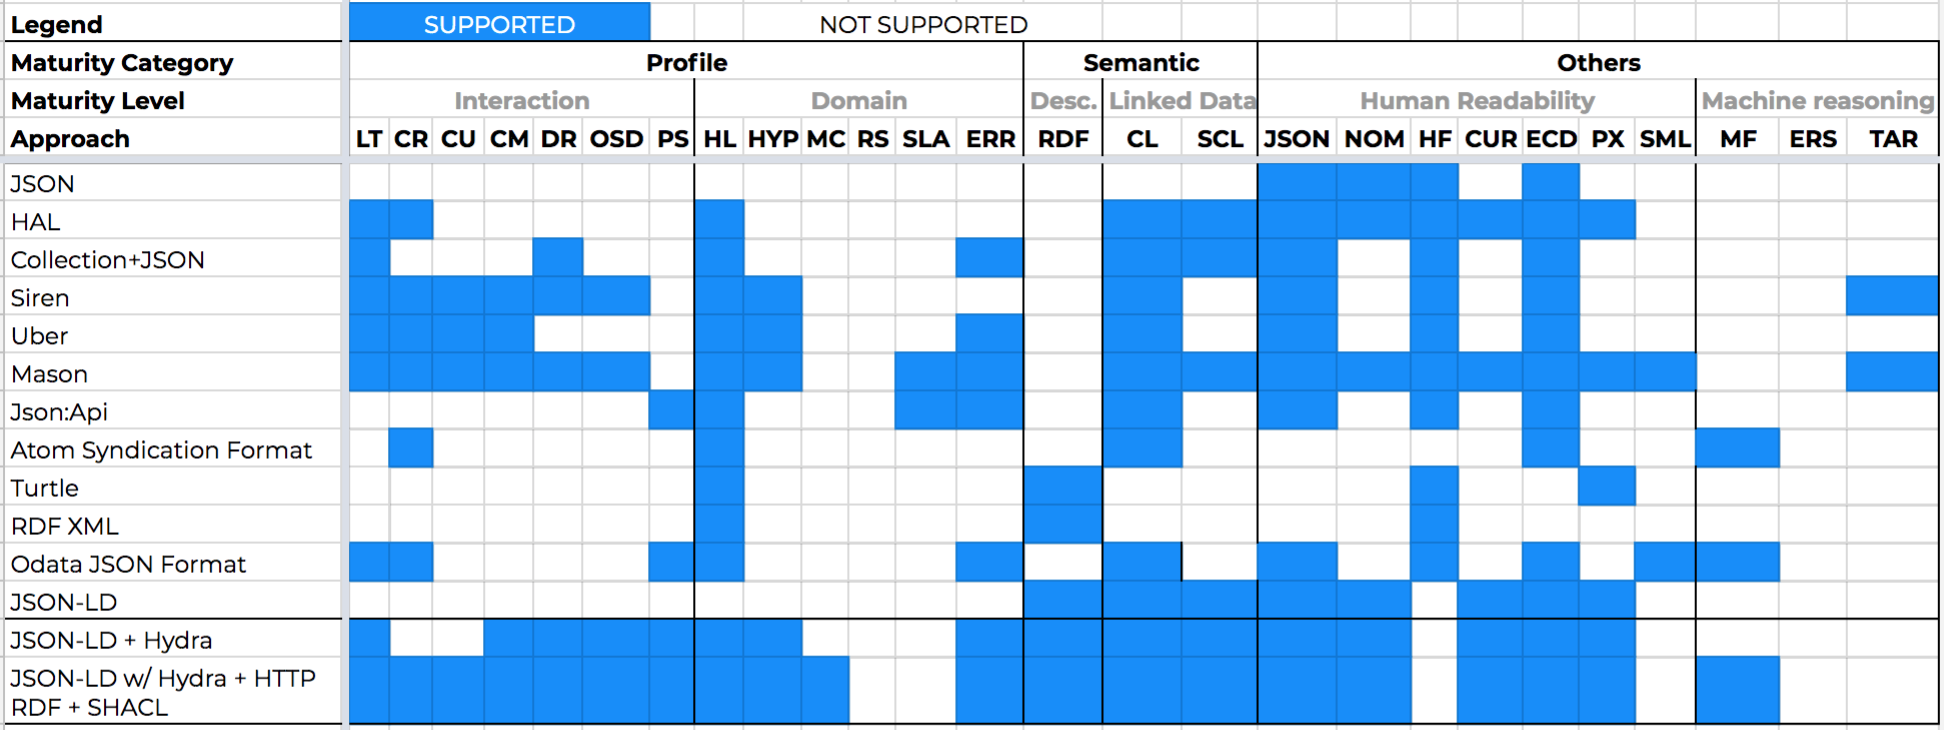
\includegraphics[width=1\textwidth]{figures/DIF.png}
\label{interchange-formats-matrix}
\end{figure*}

\subsubsection*{Synthesis}
From this matrix, we notice that formats can be differentiated based on their compatibility with RDF. Indeed, RDF formats (Turtle, RDF XML and JSON-LD) can be enriched with RDF vocabularies. This is why they propose very few features by default. To depict what is possible to achieve by combining vocabularies with a RDF format, we selected two vocabularies: Hydra and SHACL, an RDF schema validation vocabulary, that we combined with JSON-LD and evaluated. As a result, it matches 12 more criteria than JSON-LD alone.
From this, we infer that while combined with vocabularies, RDF formats allow building mature Semantic REST systems. However, this requires additional effort in order to find and select relevant vocabularies.
On the other hand, non-RDF formats help building systems that can be mature on the \textit{profile} dimension but not on the \textbf{semantic} dimension.

Last, the matrix shows that no format supports the description of constraints on the data neither the advertisement of the resource's state. Though, most scientific approaches we found describe REST APIs as state machines. Providing the resource's state would ease machine-reasoning. On the other hand, describing the constraints could decrease coupling and increase user experience. % maybe -> move to discussion

\subsection{Implementation Frameworks}

Implementation frameworks are software libraries that guide developers through the implementation of Web APIs. We limit the comparison to frameworks that claim to support HATEOAS. We identified six frameworks that do so. Frameworks to build Semantic Web Services are excluded because their approach is too far from REST.

In \cite{salvadori2014framework} authors propose \textit{Hypermedia Web API Support}, a Java framework based on JAX-RS 2.0 that uses annotations to semantically describe REST APIs. The end result is a JSON-LD document, enriched with the Hydra vocabulary, that describes the whole API. In \cite{parastatidis2010role} Parastatidis et al. present Restfulie, a framework to ease the development of REST APIs using resources, content-negotiation and state transitions as its core building blocks. Besides these frameworks, we found that API-Platform, Spring HATEOAS, JAX-RS and Ripozo support HATEOAS features. They are classified in Fig. \ref{frameworks-matrix} according to 23 criteria.

% FIGURE OF THE IMPLEMENTATION FRAMEWORKS CLASSIFICATION
\begin{figure*}[!ht]
\caption{Implementation Frameworks Comparison Matrix}
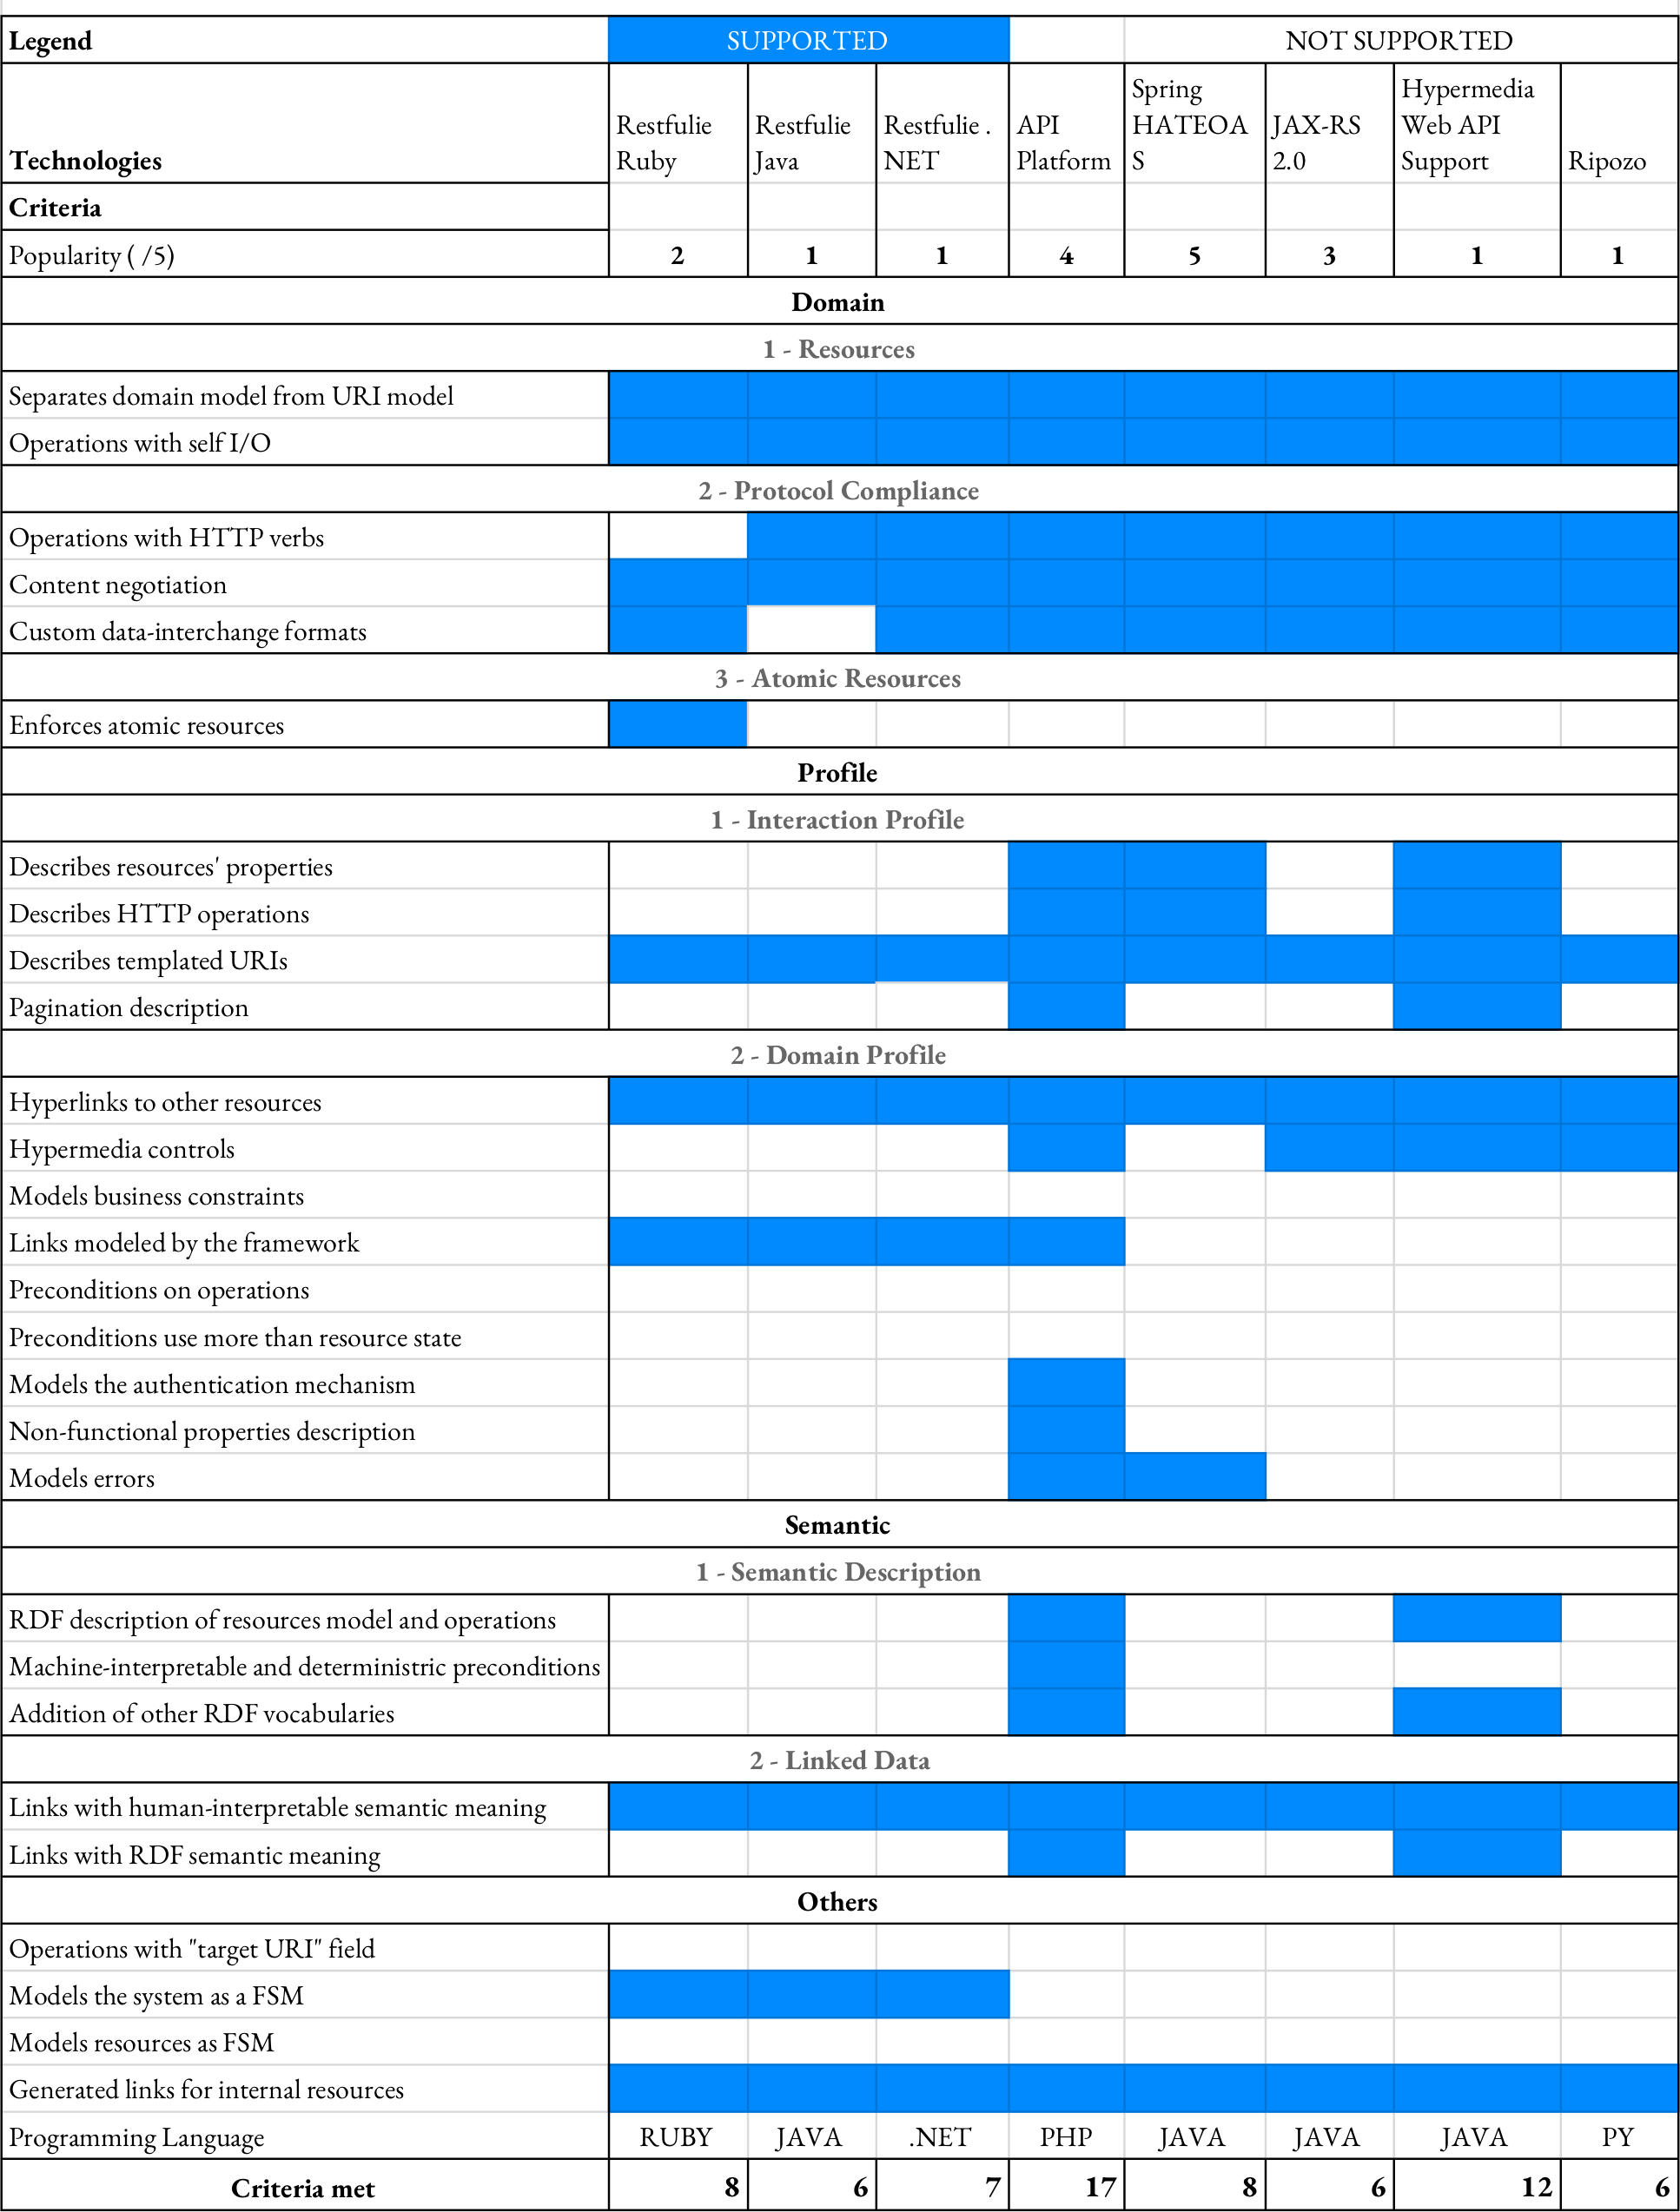
\includegraphics[width=1\textwidth]{figures/frameworks.png}
\label{frameworks-matrix}
\end{figure*}

\subsubsection*{Synthesis}
Despite the fact that only one framework enforces the \textit{Atomic Resources} constraint, all frameworks allow to reach the highest level of maturity on the Design axis easily. This is because supporting the \textit{Atomic Resources} constraint only requires developers to use the data model of the resource as the input of write operations and as the output of read operations.

We notice that only \textit{API Platform} and \textit{Restfulie} offer a mechanism to model relations between resources from which links are generated, instead of adding the links programmatically in the response, thus increasing maintainability.

Otherwise, most framework do not ease the process of semantically documenting the API. To us, this is the biggest challenge framework designers should tackle today.

Last, as for IDLs, most creators of frameworks do not provide mechanisms to describe resources as state machines, even though it could bring the same benefits.
